\documentclass[a4paper]{gretl4pydoc}
\usepackage[colorinlistoftodos,prependcaption,textsize=tiny,textwidth=2.8cm]{todonotes}

\graphicspath{{png/}}
\DeclareGraphicsExtensions{.png}

\hyphenation{libgretl}

\newcommand{\hitem}{\item[] \hspace{-5mm}}

\newcommand{\lgretl}{\pkg{libgretl}\xspace}
\newcommand{\gretl}{\pkg{gretl}\xspace}
\newcommand{\gretlpy}{\pkg{gretl4py}\xspace}
\newcommand{\python}[1][]{\proglang{Python#1}\xspace}
\newcommand{\cpp}{\proglang{C++}\xspace}
\newcommand{\installbat}{\texttt{install.bat}\xspace}
\newcommand{\estdesc}[1]{\begin{minipage}[t]{0.95\columnwidth}%
	\scriptsize#1\end{minipage}\vspace{3pt}}
% lstlistings
\newcommand{\gretlcmd}[1]{\lstinline!#1!\xspace}
\newcommand{\gretlcmdn}[1]{\inline{#1}\xspace}
\newcommand{\cppcode}[1]{\lstinline[style=cppstyle]!#1!\xspace}
\newcommand{\pythcode}[1]{\lstinline[style=pythonstyle]!#1!\xspace}
\newcommand{\reqpython}{[3.11], [3.12], [3.13]\xspace}
\newcommand{\mapto}[1]{\hspace*{17pt}maps to: \gretlcmd{#1}\newline%
	\hspace*{17pt}where \pythcode{OPTS} are the following options %
	(\gretlpy to \gretl mappings):}
\newcommand{\maptoopt}[3]{\pythcode{#1} $\rightarrow$ \gretlcmd{#2}\newline\hspace*{10pt}\footnotesize{#3}}
\newcommand{\error}[1]{\textcolor{red}{\textbf{#1}}\xspace}

\makeatletter
\@mparswitchfalse%
\makeatother

\begin{document}
	\pagestyle{headings}
	\maketitle
	\textbf{Project's main page:}
	\begin{quote}
		\centering
		\url{https://sourceforge.net/p/gretl/gretl4py}
	\end{quote}

\begin{center}
	\vspace*{100pt}{\Large Version 0.1}
\end{center}
	
%	\begin{abstract}
%		to be written...
%	\end{abstract}
	
	\tableofcontents
	
	\section*{Changelog}
	\begin{description}
		\item[0.1] Initial version.
	\end{description}

	\section*{To do}
	\begin{quote}
		\input{../todo.txt}
	\end{quote}

	\section{Introduction}
We introduce gretl4py package...

	\section{Implementation}\label{sec:implementation}

\subsection{Binary Bindings}\label{sec:binary_bindings}
The \cpp bindings are written using the \pkg{pybind11}
\citep{pybind11} package.
The main purpose of these bindings is to provide \python
interfaces to selected \lgretl estimators and utility functions
in a standardized form. Each \cpp binding has its \python
counterpart (see Section~\ref{sec:python_side} for details).

\subsubsection{Estimators}\label{sec:estimators_c++}
With \cppcode{namespace py = pybind11}:
%\lstinputlisting[style=cppstyle]{../src/gretl4py.h}

For \texttt{arma} estimation (specific case):
\begin{lstlisting}[style=cppstyle]
py::dict *arma (const std::string y, const py::tuple &tup,
								const py::kwargs &kwargs);
\end{lstlisting}

For default case:
\begin{lstlisting}[style=cppstyle]
py::dict *ESTIMATOR (const std::string formula,
								const py::kwargs &kwargs);
\end{lstlisting}
where \cppcode{ESTIMATOR} represents one of the supported
estimator functions (see Section~\error{XXX}). These bindings
return a \python dictionary (see Section~\error{XXX} for details)
and accept the following arguments:
\begin{enumerate}
	\item \cppcode{const std::string y}: The name of the dependent
		variable in a dataset (see Section~\error{XXX} for details).
	\item \cppcode{const py::tuple \&tup}: A reference to a \python
		tuple containing the SARIMA specification (see Section~\error{XXX} for details).
	\item \cppcode{const std::string formula}: A formula that constitutes
		an equation (see Section~\error{XXX} for details).
	\item \cppcode{const py::kwargs \&kwargs}: A reference to optional
		arguments (see Section~\error{XXX} for details).
\end{enumerate}


\subsection{\python Side}\label{sec:python_side}
All binary bindings described in Section~\ref{sec:binary_bindings}
have their counterparts on the \python side, with access
provided by two \python scripts: \texttt{gretl4py\_addons.py}
and \texttt{gretl4py\_classes.py}. Additionally, \gretlpy is
initialized by the \texttt{\_\_init\_\_.py} file.


\subsubsection{Estimators}\label{sec:estimators_python}
While Section~\ref{sec:estimators_c++} outlines only two
\cpp bindings, the actual list of available \lgretl estimators
is much more extensive. Keep in mind the following:
\begin{itemize}
	\item\pythcode{data=dict()} is a dictionary containing
		the data as described in~\error{XXX};
	\item\pythcode{formula=str()} can take one of the
		following forms:
		\begin{itemize}
			\item a simple \proglang{R}-style formula that
				maps the model equation using the following rule:
				\begin{center}
					\addtocounter{equation}{1}
					$\displaystyle y = \beta_0 + \sum_{j=1}^{k}\beta_jx_j + \varepsilon\;\rightarrow\;$%
					\pythcode{'y ~ const + x1 + x2 + ... + xk'}%
					\setcounter{rstylefomula}{\theequation}%
					\hfil\hypertarget{theRstyleFomula}{(\textcolor{red}{\theequation})}
				\end{center}
			\item \gretl's default syntax, as described in \cite{gretl_manual}
				and referred to here as the ``maps to'' syntax;
		\end{itemize}
\end{itemize}
The complete list of available estimators is as follows (options in square brackets are optional):

\est{ar}
\estdesc{Computes parameter estimates using the
	generalized Cochrane-Orcutt iterative procedure.}
\begin{lstlisting}[style=pythonstyle]
gretl.ar(formula=str(), [OPTS, [data=dict()]])
\end{lstlisting}
\mapto[0]{ar lags ; depvar indepvars}
\noRformula

\est{ar1}
\estdesc{Computes feasible GLS estimates for a model in which the error
	term is assumed to follow a first-order autoregressive process.}
\begin{lstlisting}[style=pythonstyle]
gretl.ar1(formula=str(), [OPTS, [data=dict()]])
\end{lstlisting}
\mapto{ar1 depvar indepvars}
\begin{itemize}
	\item[]\maptoopt{hilu=True}{--hilu}{use Hildreth–Lu procedure}
	\item[]\maptoopt{pwe=True}{--pwe}{use Prais–Winsten estimator}
\end{itemize}

\est{arima}
\estdesc{Estimates a univariate ARIMA (Autoregressive, Integrated, Moving Average) model.}
\begin{lstlisting}[style=pythonstyle]
gretl.arma(y=str(), order=tuple((p,d,q)),
	[seasonal=tuple((P,D,Q)), OPTS, [data=dict()]])
\end{lstlisting}
\mapto{arima p d q [; P D Q ] ; depvar}
\begin{itemize}
	\item[]\maptoopt{verbose=True}{--verbose}{print details of iterations}
	\item[]\maptoopt{hessian=True}{--hessian}{disables the fallback to outer
		product of the gradient (OPG)}
	\item[]\maptoopt{opg=True}{--opg}{forces use of the OPG method}
	\item[]\maptoopt{nc=True}{--nc}{do not include a constant}
	\item[]\maptoopt{conditional=True}{--conditional}{use conditional maximum likelihood}
	\item[]\maptoopt{x\_12\_arima=True}{--x-12-arima}{use X-12-ARIMA, or X13, for estimation}
	\item[]\maptoopt{lbfgs=True}{--lbfgs}{use L-BFGS-B maximizer}
	\item[]\maptoopt{lagselect=True}{--lagselect}{information criteria
		and log-likelihood for a number of AR(I)MA specifications
		are printed}
\end{itemize}

\est{ols}
\estdesc{Computes ordinary least squares (OLS) estimates with \texttt{depvar}
	as the dependent variable and \texttt{indepvars} as the list of independent variables.}
\begin{lstlisting}[style=pythonstyle]
gretl.ols(formula=str(), [OPTS, [data=dict()]])
\end{lstlisting}
\mapto{ols depvar indepvars}
\begin{itemize}
	\item[]\maptoopt{robust=True}{--robust}{robust standard errors}
	\item[]\maptoopt{jackknife=True}{--jackknife}{selecting an
		\texttt{hc\_version} of 3a, \cite[see][]{gretl_command} for details}
	\item[]\maptoopt{simple\_print=True}{--simple-print}{do not print auxiliary statistics}
	\item[]\maptoopt{no\_df\_corr=True}{--no-df-corr}{suppress degrees of freedom correction}
\end{itemize}

\est{biprobit}
\estdesc{Estimates a bivariate probit model, using
	the Newton-Raphson method to maximize the likelihood.}
\begin{lstlisting}[style=pythonstyle]
gretl.biprobit(formula=str(), [OPTS, [data=dict()]])
\end{lstlisting}
\mapto{biprobit depvar1 depvar2 indepvars1 [; indepvars2]}
\begin{itemize}
	\item[]\maptoopt{robust=True}{--robust}{robust standard errors}
	\item[]\maptoopt{opg=True}{--opg}{forces use of the OPG method}
\end{itemize}
\noRformula

\est{duration}
\estdesc{By default the Weibull distribution is used
	but the exponential, log-logistic and log-normal
	distributions are also available.}
\begin{lstlisting}[style=pythonstyle]
gretl.duration(formula=str(), [OPTS, [data=dict()]])
\end{lstlisting}
\mapto{duration depvar indepvars [; censvar ]}
\begin{itemize}
	\item[]\maptoopt{exponential=True}{--exponential}{use exponential distribution}
	\item[]\maptoopt{loglogistic=True}{--loglogistic}{use log-logistic distribution}
	\item[]\maptoopt{lognormal=True}{--lognormal}{use log-normal distribution}
	\item[]\maptoopt{robust=True}{--robust}{robust standard errors}
	\item[]\maptoopt{verbose=True}{--verbose}{print details of iterations}
\end{itemize}

\est{garch}
\estdesc{Estimates a GARCH model, either a univariate
	model or, if indepvars are specified, including the
	given exogenous variables.}\todo{\texttt{fcp} option must be verified}
\begin{lstlisting}[style=pythonstyle]
gretl.garch(formula=str(), [OPTS, [data=dict()]])
\end{lstlisting}
\mapto{garch p q ; depvar [indepvars]}
\begin{itemize}
	\item[]\maptoopt{robust=True}{--robust}{robust standard errors}
	\item[]\maptoopt{nc=True}{--nc}{do not include a constant}
	\item[]\maptoopt{stdresid=True}{--stdresid}{standardize the residuals}
	\item[]\maptoopt{arma\_init=True}{--arma-init}{initial variance parameters from ARMA}
\end{itemize}
\noRformula

\est{heckit}
\estdesc{Heckman-type selection model. In the specification,
	the list before the semicolon represents the outcome equation,
	and the second list represents the selection equation. The
	dependent variable in the selection equation (ys in the
	example above) must be a binary variable.}
\begin{lstlisting}[style=pythonstyle]
gretl.heckit(formula=str(), [OPTS, [data=dict()]])
\end{lstlisting}\todo{formula rendering must be fixed}
\error{Formula rendering failed}

\est{lad}
\estdesc{Calculates a regression that minimizes the sum of
	the absolute deviations of the observed from the
	fitted values of the dependent variable.}
\begin{lstlisting}[style=pythonstyle]
gretl.lad(formula=str(), [OPTS, [data=dict()]])
\end{lstlisting}
\mapto{lad depvar indepvars}
\begin{itemize}
	\item[]\maptoopt{no\_vcv=True}{--no-vcv}{don't compute covariance matrix}
\end{itemize}

\est{logistic}
\estdesc{Logistic regression: carries out an OLS
	regression using the logistic transformation
	of the dependent variable.}\todo{\texttt{ynax} option must be verified}
\begin{lstlisting}[style=pythonstyle]
gretl.logistic(formula=str(), [OPTS, [data=dict()]])
\end{lstlisting}
\mapto{logistic depvar indepvars}
\begin{itemize}
	\item[]\maptoopt{robust=True}{--robust}{robust standard errors}
	\item[]\maptoopt{fixed\_effects=True}{--fixed-effects}{estimate with group fixed effects}
\end{itemize}

\est{logit}
\estdesc{By default the slopes with respect to each of
	the independent variables are calculated (at the means
	of those variables) and these slopes replace the usual
	p-values in the regression output.}
\begin{lstlisting}[style=pythonstyle]
gretl.logit(formula=str(), [OPTS, [data=dict()]])
\end{lstlisting}
\mapto{logit depvar indepvars}
\begin{itemize}
	\item[]\maptoopt{robust=True}{--robust}{robust standard errors}
	\item[]\maptoopt{multinomial=True}{--multinomial}{estimate multinomial logit}
	\item[]\maptoopt{verbose=True}{--verbose}{print details of iterations}
	\item[]\maptoopt{p\_values=True}{--p-values}{show p-values instead of slopes}
	\item[]\maptoopt{estrella=True}{--estrella}{select pseudo-R-squared variant}
\end{itemize}

\est{mpols}
\estdesc{Computes OLS estimates for the specified model using multiple
	precision floating-point arithmetic.}
\begin{lstlisting}[style=pythonstyle]
gretl.mpols(formula=str(), [OPTS, [data=dict()]])
\end{lstlisting}
\mapto[0]{mpols depvar indepvars}

\est{negbin}
\estdesc{Estimates a Negative Binomial model. The dependent
	variable is taken to represent a count of the occurrence
	of events of some sort, and must have only non-negative
	integer values.}
\begin{lstlisting}[style=pythonstyle]
gretl.negbin(formula=str(), [OPTS, [data=dict()]])
\end{lstlisting}
\mapto{negbin depvar indepvars}
\begin{itemize}
	\item[]\maptoopt{model1=True}{--model1}{use NegBin 1 model}
	\item[]\maptoopt{robust=True}{--robust}{QML covariance matrix}
	\item[]\maptoopt{opg=True}{--opg}{forces use of the OPG method}
	\item[]\maptoopt{verbose=True}{--verbose}{print details of iterations}
\end{itemize}

\est{panel}
\estdesc{By default the fixed effects estimator is used; this is implemented
	by subtracting the group or unit means from the original data.}
\begin{lstlisting}[style=pythonstyle]
gretl.panel(formula=str(), [OPTS, [data=dict()]])
\end{lstlisting}
\mapto{panel depvar indepvars}
\begin{itemize}
	\item[]\maptoopt{fixed\_effects=True}{--fixed-effects}{estimate with group fixed effects}
	\item[]\maptoopt{random\_effects=True}{--random-effects}{random effects or GLS model}
	\item[]\maptoopt{nerlove=True}{--nerlove}{use the Nerlove transformation}
	\item[]\maptoopt{pooled=True}{--pooled}{estimate via pooled OLS}
	\item[]\maptoopt{between=True}{--between}{estimate the between-groups model}
	\item[]\maptoopt{robust=True}{--robust}{robust standard errors \cite[see][]{gretl_command}}
	\item[]\maptoopt{unit\_weights=True}{--unit-weights}{weighted least squares}
	\item[]\maptoopt{iterate=True}{--iterate}{iterative estimation}
	\item[]\maptoopt{matrix\_diff=True}{--matrix-diff}{compute Hausman test via matrix difference}
\end{itemize}

\est{poisson}
\estdesc{The dependent variable is taken to represent the occurrence
	of events of some sort, and must take on only non-negative integer values.}
\begin{lstlisting}[style=pythonstyle]
gretl.poisson(formula=str(), [OPTS, [data=dict()]])
\end{lstlisting}
\mapto{poisson depvar indepvars [; offset]}
\begin{itemize}
	\item[]\maptoopt{robust=True}{--robust}{robust standard errors}
\end{itemize}
\noRformula

\est{probit}
\estdesc{By default the slopes with respect to each of
	the independent variables are calculated (at the means
	of those variables) and these slopes replace the usual
	p-values in the regression output.}
\begin{lstlisting}[style=pythonstyle]
gretl.probit(formula=str(), [OPTS, [data=dict()]])
\end{lstlisting}
\mapto{probit depvar indepvars}
\begin{itemize}
	\item[]\maptoopt{robust=True}{--robust}{robust standard errors}
	\item[]\maptoopt{verbose=True}{--verbose}{print details of iterations}
	\item[]\maptoopt{p\_values=True}{--p-values}{show p-values instead of slopes}
	\item[]\maptoopt{estrella=True}{--estrella}{select pseudo-R-squared variant}
	\item[]\maptoopt{random\_effects=True}{--random-effects}{estimates a random effects panel probit model}
\end{itemize}

\est{tsls}
\estdesc{Computes Instrumental Variables (IV) estimates,
	by default using two-stage least squares (TSLS).}
\begin{lstlisting}[style=pythonstyle]
gretl.tsls(formula=str(), [OPTS, [data=dict()]])
\end{lstlisting}
\mapto[0]{tsls depvar indepvars ; instruments}\todo{formula rendering must be fixed}
\error{Formula rendering failed}

\est{wls}
\estdesc{Computes weighted least squares (WLS) estimates
	using \texttt{wtvar} as the weight, \texttt{depvar}
	as the dependent variable, and \texttt{indepvars}
	as the list of independent variables.}\todo{\texttt{allow\_zeros} option must be verified}
\begin{lstlisting}[style=pythonstyle]
gretl.wls(formula=str(), [OPTS, [data=dict()]])
\end{lstlisting}
\mapto{wls wtvar depvar indepvars}
\begin{itemize}
	\item[]\maptoopt{robust=True}{--robust}{robust standard errors}
	\item[]\maptoopt{allow\_zeros=True}{--allow-zeros}{to mix zero weights with positive ones}
\end{itemize}
\noRformula

	\section{Installation}
\subsection{System Requirements}
Before installing or compiling \gretlpy, please ensure
the following components are installed:
\begin{itemize}
	\item One of the supported versions of \python: (\reqpython);
	\item The following required \python packages: \pkg{csv},
		\pkg{json}, \pkg{numpy}, \pkg{pandas}, and \pkg{subprocess};
	\item \gretl (refer to \url{https://gretl.sourceforge.net} for details)%
		\footnote{Note: For MS Windows, the UCRT build is required. See:
			\url{https://sourceforge.net/projects/gretl/files/snapshots/}.};
\end{itemize}

\subsection{Native MS Windows}
The easiest way to install \gretlpy on a Windows machine is
by running the \installbat script from the \gretlpy root
directory. The script assumes that \texttt{python.exe} is
available in the current \texttt{PATH}. If this is not the case,
please modify \installbat accordingly. Additionally, the script
assumes that \gretl is installed in the default location, i.e.,
\texttt{C:\textbackslash Program Files\textbackslash gretl}. If
this is not the case, please modify \texttt{gretl4py\_env.bat}
or \texttt{gretl4py\_env.ps1} as needed.

The \installbat script will copy the following files into the
path generated by the command: \texttt{python.exe -m site --user-site}:

\begin{itemize}
	\item \texttt{\_\_init\_\_.py}, \texttt{gretl4py\_addons.py},
		and \texttt{gretl4py\_classes.py} from the \texttt{[gretl]} directory;
	\item \texttt{\_gretl.cp3xx-win\_amd64.pyd} from the
		\texttt{[builds\textbackslash win64\textbackslash 3.xx]} directory;
	\item \texttt{glib-2.0.dll} and \texttt{libintl-8.dll} from the
		\texttt{[builds\textbackslash win64\textbackslash DLL]} directory%
		\footnote{This is a temporary solution, and the copying of these
			two files will be removed in a future update.};
\end{itemize}

In this context, \texttt{3.xx} refers to the version of \python being used.
Figure~\ref{fig:mswindows_install.bat} shows an example output from \installbat.

\begin{figure}[h]
	\centering
	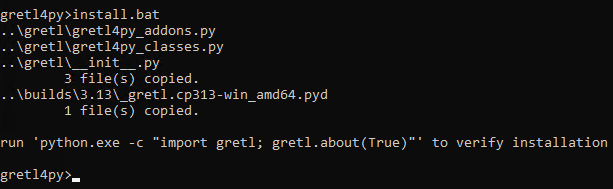
\includegraphics[width=.75\columnwidth,keepaspectratio]{mswindows_install.bat}
	\label{fig:mswindows_install.bat}
	\caption{Example output from \installbat}
\end{figure}

	\section{Usage of the package}
\error{A description of scripts in \texttt{demo} directory goes here}

	\section{Examples}
\error{to be written$\ldots$}

\section{\gretlpy as \pkg{statsmodels} replacement}
\error{to be written$\ldots$}

	
	\bibliographystyle{abbrvnat}
	\bibliography{gretl4py.bib}
\end{document}
